%\chapter{Introduction1}
%\minitoc \mtcskip \noindent
%\chapter{Introduction2}
%\minitoc \mtcskip \noindent
\chapter{Introduction}
\label{chap:introduction}
\minitoc \mtcskip \noindent

Our society is turning more consumerist, with most people in developed countries having high consumer power and standards of life. Consumers goods, from the essentials up until the entertainment goods, are manufactured and ordered continuously in high quantities.

Modern supply chains feel the pressure of this growth, leading to the demand for an efficient management. Most companies are making efforts towards this end, and, even though part of the answer to an efficient management lies in having efficient processes, a good management is also based in using the right technologies. Thus, the development of technologies that can satisfy the demands of supply chain management, for any industry, is in high demand.

%The development of such technologies should be faced towards the problems that supply chains 

%ace concerns are raised as to whether the demand can be met in a transparent and trustful way. It is difficult to know where the products we consume come from, and the processes they go through. This leads to the need of transparency in the supply chains as well as the need of an increase in their efficiency, if they are to conform to the market's needs.

\section{Supply Chains}
\label{supply_chains}
\textbf{Supply Chains} can be found, in some form, in nearly every business, spanning many different areas of operation. Traditionally, a supply chain encompasses all the processes and activities that lead from the initial raw materials to the final finished product, as well as all the functions and services within and outside a company. A supply chain can also be defined as the network of entities through which material flows. These entities can be identified as suppliers, carriers, manufacturing sites, distribution centers, retailers, and customers~\cite{Lummus2014}. Naturally, with the upstream and downstream flow of these materials and resources, comes a lot of information on them and on the processes, people and organizations they are associated with. Realistically, the  flow is not always arborescent, as there are many considerations to be taken and decisions to be made. Supply chains have multiple end products with shared components, facilities and capacities~\cite{Ganeshan1995}. As a consequence, the paths taken by the resources and information are not straightforward, but interlace, diverge and converge at different points, go back and forth, as exemplified in Figure~\ref{fig:supplychain_complexity}.
  
\begin{figure}[ht]
\centering
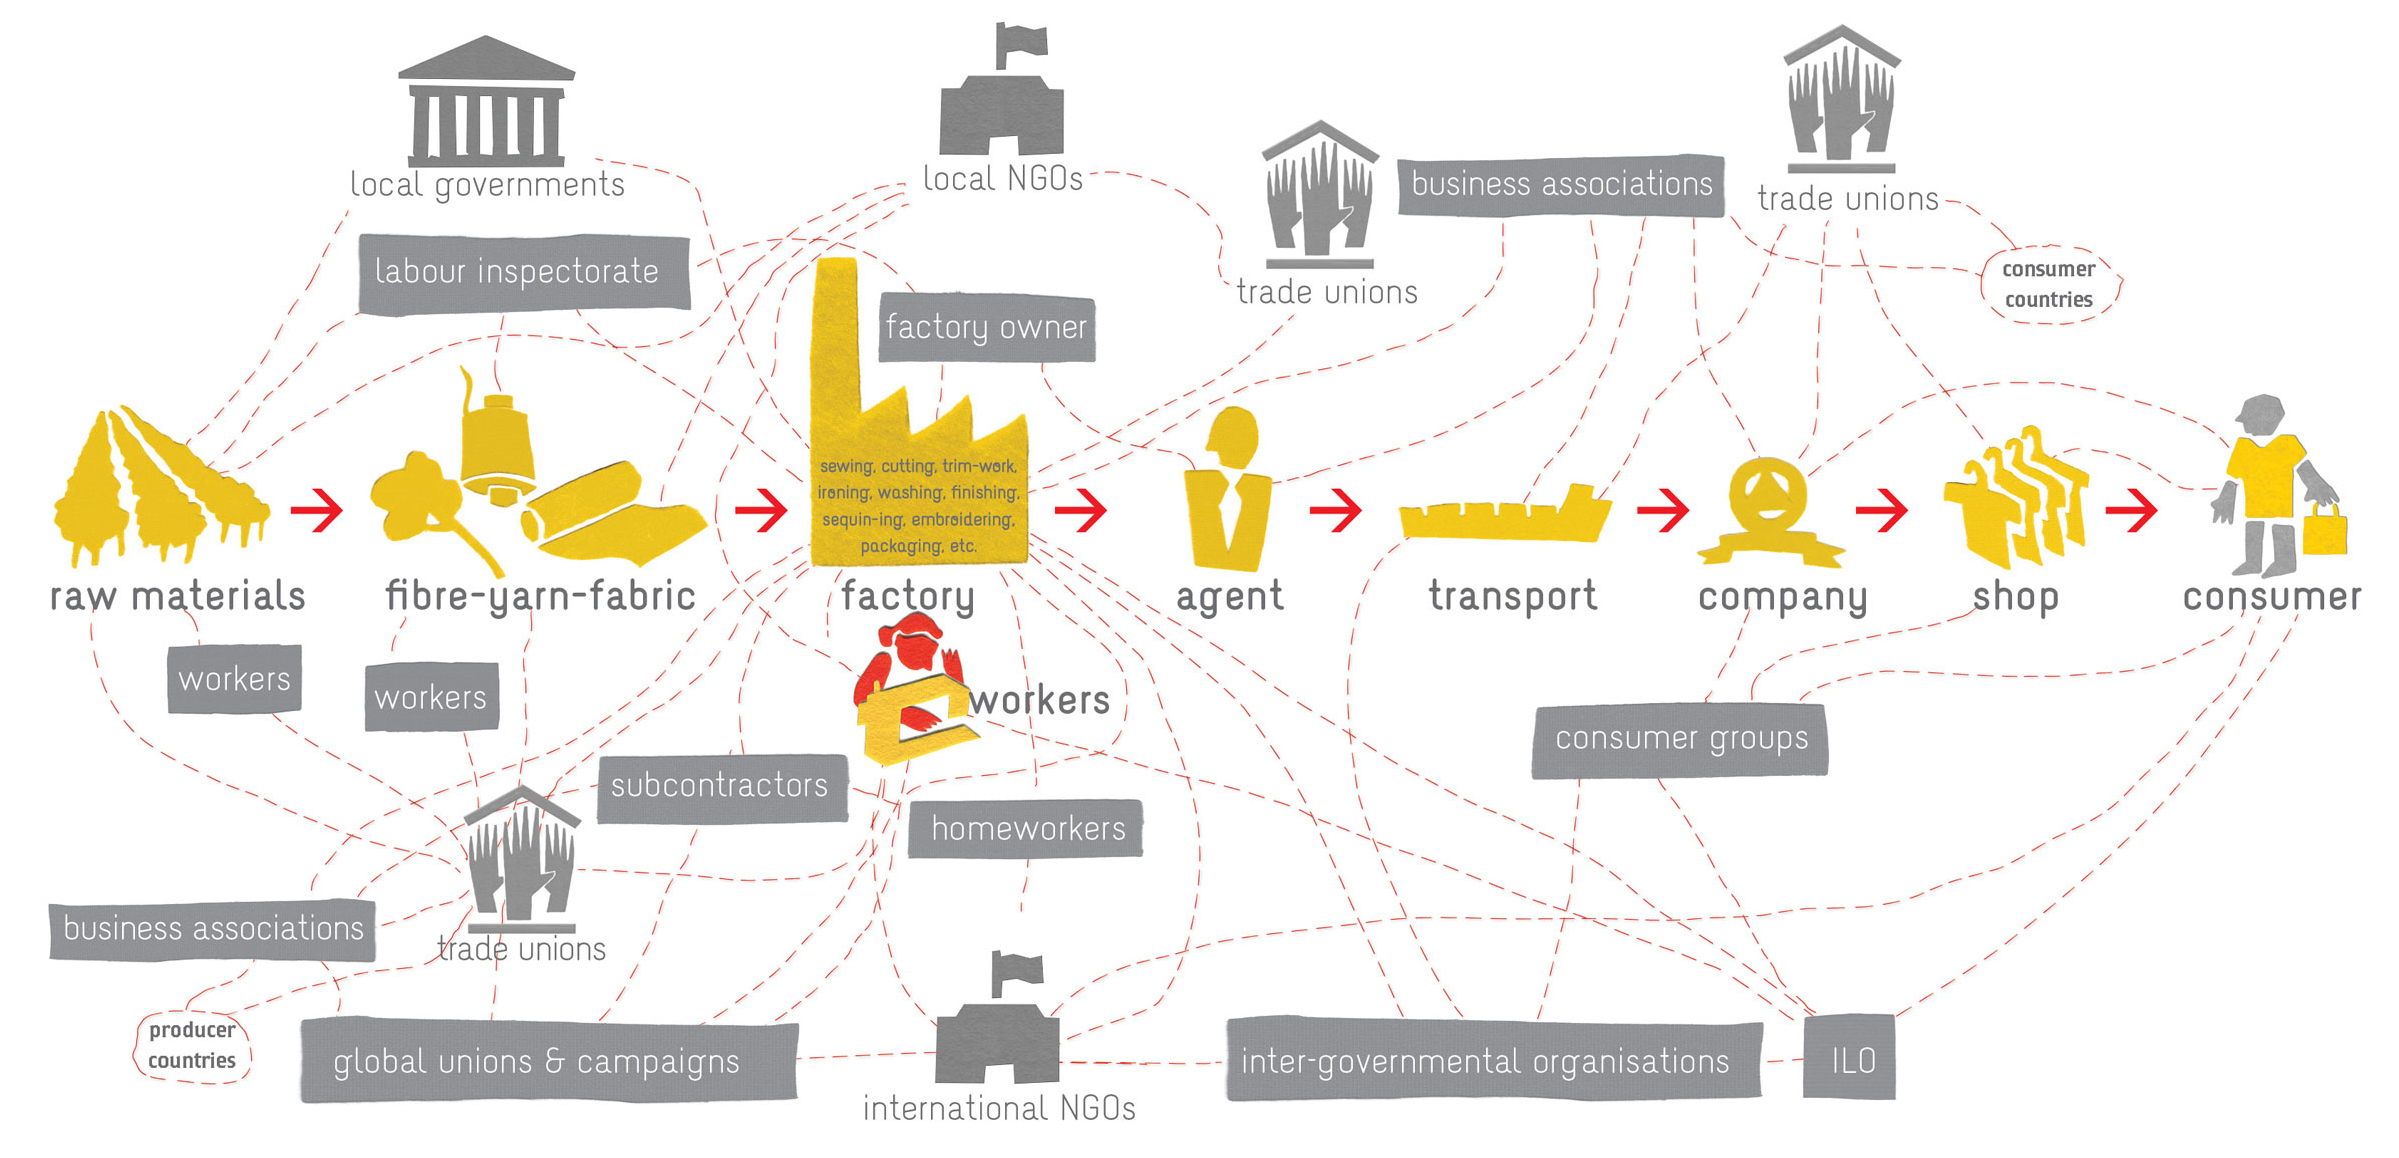
\includegraphics[scale=0.18]{media/supplychain_complexity.jpg}
\caption[Representation of a garment supply chain and all the relationships it involves]{Representation of a garment supply chain and all the relationships it involves. Taken from the International Training Centre of the International Labour Organization briefing on global supply chains~\cite{ITCILO2018}.}
\label{fig:supplychain_complexity}
\end{figure}
  
  The activities and processes a supply chain encompasses include: sourcing raw materials and parts, manufacturing and assembly, warehousing and inventory tracking, order entry and order management, distribution across all channels, delivery to the customer, and managing the information systems necessary to monitor all of these activities. As Lummus~\cite{Lummus2014} describes, these activities can be roughly mapped to the 4 essential processes: plan, source, make, deliver.
    
  Coordinating all of these is no easy task, and so the discipline of SCM comes into life. According to Ballou~\cite{Ballou2007}, the Council of SCM Professionals (CSCMP) defines SCM as \textit{“the planning and management of all activities involved in sourcing and procurement, conversion, and all Logistics Management activities. Importantly, it also includes coordination and collaboration with channel partners, which can be suppliers, intermediaries, third-party service providers, and customers. In essence, SCM integrates supply and demand management within and across companies”}.

From this definition follows that SCM deals a lot with both coordination and collaboration between entities, and so, the management of the flow of information and resources between them is very important. The objective is always, of course, to minimize the total cost of these flows between and among stages~\cite{Habib2011}.
In the end, the creation of value (products and services) in a supply chain stems from the relationships that different entities build between themselves, and not from the work of a single entity. As such, supply chains, not firms, compete and those which have the best integration and management processes win.

And this is where SCM shines and shows just how useful it can be. Managing all the processes in a supply chain, while maintaining safety, quality and keeping to schedule is difficult. An event on one side of the world, large or small, be it from human or natural causes, can easily disrupt the links in the supply chain. For instance, it might disrupt the supply of a critical component or service. Delays are, therefore, common, and the consequences of such disruptions might have a severe impact in the finances, growth and reputation of the companies involved~\cite{Punter2013}.

SCM diminishes the impact of such disruptions, and actively works to avoid or diminish them, while optimizing the way the supply chain works. This is why SCM is such an important discipline, that we have to better understand and improve, with all the means that we can, and this includes, of course, research into technologies like the blockchain.

\section{Challenges}
\label{sec:supply-chain-challenges}

 Having already introduced the concepts of Supply Chain and SCM, it is now possible to briefly introduce some of the problems that affect them.

The first, and most generalist problem of a supply chain, is the ease with which \textbf{an unexpected event might cause delays}. These events, already mentioned in Section~\ref{supply_chains} are not always predictable and must be contained as fast as possible. One event in particular which, often, causes delays are \textbf{synchronization problems in the processes and information systems of a company}~\cite{Prokle2017}. 

    Another problem is that, often, there are difficulties in sharing information between companies. This is caused both by the fact that \textbf{companies value their privacy and the security of their information}, which means they might not want to share too much information, or that they might only share it through secure channels, and by the \textbf{lack of standards for sending information and communicating}~\cite{Korpela2017}. The issue with non-existing standards is that companies are left to discuss what details to share or not, wasting time and resources.

Most important of all, in the industry, \textbf{the use of traditional tools and manual work is still too prevalent}. Emails are sent, documents are printed and mailed, instead of transmitting the information in a more automatic, direct and secure way through the network. This point also brings the next problem of supply chains to light: the apparent lack of interoperability between certain softwares (which might be a byproduct of by the lack of standards).
 
 
Finally, provenance and traceability of the products on a supply chain are a big objective for companies. But \textbf{the current technologies used in supply chain only accomplish provenance and traceability in a limited scope}, as the information a certain entity possesses is usually also limited. And so, it is very hard for anyone to have a global overview of the supply chain.

Though it is not proven, it is be possible that some, if not most, of these issues in supply chain might be caused by the use of software architectures that do not allow for full data integration. An optimal supply chain should be as efficient and effective as possible, while being secure and satisfying all the traceability requirements. Perhaps, it is time to try out new solutions which replace or augment the existing ones, in such a way that supply chain management can better satisfy the needed requirements.

\section{From Blockchain Technologies to Supply Chains} \label{sec:context}

Blockchain technology allows for secure, public, distributed and decentralized systems. Though it was first proposed in its actual form by Satoshi Nakamoto~\cite{Nakamoto2008}, an anonymous group which published a white paper in 2008, this was not the first reference to such a technology. The first work on a cryptographically secured chain of blocks was described in 1991 by Stuart Haber and W. Scott Stornetta~\cite{Haber1991}, and further refined in 1992 by Bayer \& Haber, by incorporating Merkle trees~\cite{Bayer1993}. Since then, it has come a long way, sprouting multiple different uses and applications of the technology. Its characteristics make the development of distributed and permanently, globally available systems possible, which is a paradigm that is attracting the interest of various industries.

One area in particular where we believe blockchain could bring about great improvements is Supply Chain Management (SCM). SCM has seen an increase in complexity in the last few decades, due to the globalization of the market, with businesses interlacing in many different ways, their relations extending way beyond what they used to, as found by Filiz Isik~\cite{Isik2011}. This increase in complexity is somewhat hard to manage and some supply chains stretch and encompass so many businesses that, due to their software not being prepared for this, the information is not always transmitted from end to end, leaving holes of information in between the links that join each business, thus leading to a lot of chaos and uncertainty as to the state of the key items in the chain~\cite{Wilding1998}.

   This dissertation work will focus on supply chain management, and on how blockchains can possibly be applied to improve this area, leading to positive impacts in the logistics industry and eventually finding benefits for the consumer as well. 

%%%%%%%%%%%%%%%%%%%%%%%%%%%%%%%%%%%%%%%%%%%%%%%%%%%%%%%%%%%%%%%%%%%

\section{Motivation} 
\label{sec:motivation}

As described in section~\ref{sec:supply-chain-challenges}, a possible cause of these problems might be the use of software that can not keep up with the evolution of the requirements of modern supply chains. Today's supply chains have high standards for their requirements and even when the software works just fine, maybe it is not recent enough or it was not specified and built to satisfy these requirements. For instance, product falsification might be a huge issue nowadays in the supply chain, but maybe it was not rated as a high importance problem 15 years ago. Therefore, the software from 15 years ago complied with different requirements than the ones from today and was not built to handle that specific problem well. 

\textbf{Requirements evolve, and so should the technology, in order to support them.} There is an immediate need for solutions, which might either completely replace the previous ones, or augment them.

One way to approach these specific problems is to research what would a modern requirements specification for supply chain look like, and develop new technologies that are more accurately specified for the supply problem challenges in question. 

The characteristics of blockchain architectures seem to be a good solution for many of the identified problems in supply chain to be reduced or neutralized. These architectures are the perfect means to achieve traceability of a supply chain, and so, they are good to achieve provenance as well. At the same time they are a secure, incorruptible and immutable way to store information, with a fast synchronization time, being perpetually available to anyone who has permission, anywhere within the network. It would also be the way to close the analog gaps, turning the chain fully digital, leading to the possibility of a global overview.

\section{Objectives}
\label{sec:objectives}
The main objective of this dissertation is to find whether blockchain technology is a good fit to solve the most common problems of supply chain management, and also to find out the technological requirements of a modern supply chain. There are a multitude of small tasks that blockchain could automatize in supply chain, so this thesis will try to figure out which ones blockchain applies to better. 

The primary objective of this dissertation is determining if blockchain architectures can be successfully applied to supply chain management as an improvement towards the technologies that are already being used. For this purpose, it is necessary to conduct research on the supply chain issues and validate these, in order to propose a blockchain design that can target these issues successfully. 

\section{Dissertation Structure} \label{sec:struct}

Besides the introduction, this dissertation has 6 more chapters, divided into 2 parts.

\par \textbf{Part 1: Background and State of the Art} - Provides the needed concepts to understanding the work, as well as explanations about the existing tools and projects related to the blockchain and to its application to supply chain management domain.
 The state of the art is divided into 2 chapters:~\ref{chap:blockchain} and ~\ref{chap:blockchain-applicability}.
\begin{itemize}
  \item Chapter~\ref{chap:blockchain}, "Blockchain Technologies", some important concepts from the blockchain architecture are presented and discussed, followed by an analysis of the existing blockchain networks and frameworks and their comparison.
  \item Chapter~\ref{chap:blockchain-applicability}, "Blockchain in the Industry", the application of blockchain to supply chain is discussed in more detail, including the possible advantages, challenges, and following it up with an analysis of the existing blockchain applications that also focus on supply chain. 
\end{itemize}

\par \textbf{Part 2: Problem, Research and Solution} - Provides a thorough explanation of the problem, objectives and the proposed methodology to approach them. Follows up with a survey and requirements analysis, which serves as a base to propose a blockchain solution design. 
\begin{itemize}
  \item Chapter~\ref{chap:supply-chain-problems}, "Problem Statement", specifies the thesis statement and the questions that need to be answered in order to reach a conclusion.
  \item Chapter~\ref{chap:survey}, "Supply Chain Issues Validation and Requirements Elicitation", features a survey and the analysis of its results, such as to gather the requirements for a supply chain system, so that a blockchain-based solution can be proposed.
  \item Chapter~\ref{chap:prototype}, "Solution Design and Implementation", features the choice of a blockchain framework and the proposal of a solution, which consists in building a proof of concept (PoC) project that implements the requirements elicited from the survey.
\end{itemize}

\par \textbf{Part 3: Conclusion} - Gathers all the information from the results of the solution to make a statement, also listing contributions, difficulties and future work.
\begin{itemize}
  \item Chapter~\ref{chap:conclusions}, "Conclusions", features an overview of the work done in the dissertation, providing an answer to the previously defined problem, and following it up with possibilities of future work in this area.
\end{itemize}